\chapter{The Special Theory of Relativity}\label{c1}
\begin{enumerate}
\item A frame of reference is a set of cartesian coordinate axes and 
synchronised clocks at each point in the space.

\item An inertial frame is the one in which Newton's first law is valid. The 
existence of such frames was inferred from the experimental observations of the
seventeenth and the eighteenth centuries.

\item Experiments also showed that a frame fixed to the earth is not inertial
but the one fixed with respect to the distant stars was. If $K$ is an inertial
frame then so is $K^\op$ if it moves at a constant velocity relative
to $K$. Thus, there are an infinite number of inertial frames.

\item Consider two inertial frames of reference $K$ and $K^\op$. Let $\vec{r}$
and $\vec{r}^\op$ be the position vectors of a particle in the two frames. If 
$\vec{v}$ and $\vec{v}^\op$ are the velocities of the particle then $\vec{v} =
\vec{v}^\op + \vec{v}_0$, where $\vec{v}_0$ is the constant relative velocity
of $K^\op$ with respect to $K$.

Suppose that the particle is at position $\vec{r}_1$ at time $t_1$ and 
$\vec{r}_2$ at time $t_2$ in frame $K$. If the corresponding positions are
$\vec{r}_1^\op$ and $\vec{r}_2^\op$ in $K^\op$ then
\begin{eqnarray*}
\vec{r}_1 &=& \vec{v}_0t_1 + \vec{r}_1^\op(t_1) + \vec{r}_0 \\
\vec{r}_2 &=& \vec{v}_0t_2 + \vec{r}_2^\op(t_2) + \vec{r}_0
\end{eqnarray*}
If $\delta t = t_2 - t_1, \delta\vec{r} = \vec{r}_2 - \vec{r}_1, 
\delta\vec{r}^\op = \vec{r}_2^\op - \vec{r}_1^\op$ then
\[
\delta\vec{r} = \vec{v}_0\delta t + \delta\vec{r}^\op.
\]
If $\vec{v}_0 = \delta\vec{r}/\delta t$ then $\delta\vec{r}^\op = 0$. Thus, if
an event happens are point $\vec{r}_1$ at time $t_1$ in $K$ and another one
happens at $\vec{r}_2$ at time $t_2 = t_1 + \delta t$ then the two events 
happen at the same place in $K^\op$ if $\delta\vec{r}/\delta t$ is the relative
velocity of $K^\op$ with respect to $K$. Whether or not two events happen at
the same place thus depends on the frame of the observer.

\item This idea can be corroborated by a simple example. An person on a platform
may see a passenger lifting a tea cup as the coach entered the platform and take
it to his lips as the coach exited it. The two events thus occurred, from his 
perspective, at different points. However, a co-passenger will report them to
be happening at the same spot. The observers will agree on the duration between
the events.

\item The special theory of relativity has its roots in two facts borne out 
of experiments:
\begin{itemize}
\item The laws of physics are the same in all inertial frames of reference and
\item Changes in the state of a system are propagated with a finite speed.
\end{itemize}

\item It is also confirmed by experiments that the changes in the state of 
system are propagated at a speed not exceeding
\begin{equation}\label{c1e1}
c = 2.998 \times 10^{10} \;\text{cm/s}.
\end{equation}
No material body can move at a speed exceeding $c$ because if it could then it
can be used to signal the change of state of another body. Further, $c$ is the
maximum speed in \emph{all} inertial frames. For if it were not then the laws of
physics will not be identical across frames. Thus, $c$ is a universal constant.
It is also the speed of light in vacuum.

\item The idea of an absolute, universal time is in conflict with the 
experimental observation of a finite speed of propagation of light in vacuum. 
For if the speed is $c$ in a frame $K$ then its speed will be $3c/2$ in a frame 
$K^\op$ approaching $K$ with a speed $c/2$ in a direction opposite to that of 
propagation of light. That this is not true was confirmed by Michelson and 
Morley's experiment.  Time elapses differently in different systems and 
therefore a value of a time difference must be accompanied by a specification 
of the frame in which it was measured.

\item Consider a frame $K$ with a source of light at its origin and two 
detectors at points $(-a, 0)$ and $(a, 0)$. A spherical light front will reach 
the two detectors simultaneously when observed from $K$. Let us consider the 
experiment replicated in another frame $K^\op$ that moves with a velocity 
$v\uv{x}$ with respect to $K$. Suppose that their origins coincided then the 
light signal was emitted in $K$. Since the speed of light is the same in $K$ 
and $K^\op$ an observer in $K^\op$ also sees a spherical wavefront propagating 
isotropically. However, he will observe the wavefront reaching $(a, 0)$ sooner 
than it reaches $(-a, 0)$.  Events that are simultaneous in $K$ are not so in 
$K^\op$.

Instead of a light pulse, if two balls were fired simultaneously from the 
centre of the coach with the same speed then the observer in $K$ will once 
again conclude that they hit the edges of the coach at the same time. If $2L$
is the length of the coach, they travel a distance $L$ in time $\delta t =L/u$.
An observer in $K^\op$ sees the ball moving forward with speed $v + u$. In
time $\delta t$, it covers a distance $(v + u)\delta t$ while the front edge
recedes by a distance $v\delta t$. The relative distance between the ball and
the edge is $L + v\delta t - (v + u)\delta t$. When it becomes zero, the ball
fits the front edge. It happens at a time $L = u\delta t$. This is the same
duration as measured in $K^\op$. The ball moving towards the rear end is 
seen to be moving at a velocity $(v - u)\uv{x}$. In a time $\delta t$, it 
suffers a displacement of $(v - u)\delta t\;\uv{x}$ while the rear edge 
approaches it be a distance $v\delta t\uv{x}$. The relative distance between the
rear edge and the ball moving towards it is $L - v\delta t + (v - u)\delta t$.
Once again, the relative distance vanishes at $\delta t = L/u$. Thus an 
observer in $K$ also sees the balls hitting the edges of the coach 
simultaneously.

\item An event is described by the point at which it occurred and the time when 
it occurred. The four numbers describing an event can be interpreted as points 
in a four-dimensional space. They are called the \emph{world points}. World 
points of a system move along curves in the four-dimensional space called the 
\emph{world lines}.

\item A material body at a point $\vec{r}$ to which nothing happens travels 
along a world line that is parallel to the $t$ axis. In the four-dimensional 
space, nothing is still. If a material body moves along the $x$ axis with a 
uniform speed $v$ then its world line is a straight line making an angle 
$\tan^{-1}(v)$ with the $t$ axis. If it accelerates (decelerates) then the 
world line will be a curve turning towards (away from) the $x$-axis. 
\begin{figure}
\includegraphics[scale=0.8]{ex1}
\caption{World lines}
\label{c1f1}
\end{figure}

\item Consider an experiment in an inertial frame in which light took time 
$\delta t$ to travel between points $(x, y, z)$ and $(x + \delta x, y + 
\delta y, z + \delta z)$. The same experiment was observed from another inertial 
frame in which the light pulse travelled from $(x^\op, y^\op, z^\op)$ to $(x^\op 
+ \delta x^\op, y^\op + \delta y^\op, z^\op + \delta z^\op)$ in time $\delta 
t^\op$.  Since the speed of light is the same in two frames,
\begin{eqnarray}
c^2\delta t^2 &=& \delta x^2 + \delta y^2 + \delta z^2 \label{c1e2} \\
c^2\delta {t^\op}^2 &=& \delta {x^\op}^2 + \delta {y^\op}^2 + \delta {z^\op}^2 
\label{c1e3}
\end{eqnarray}
From these equations, we conclude that
\begin{equation}\label{c1e4}
c^2\delta t^2 - \delta x^2 - \delta y^2 - \delta z^2 = 
c^2\delta {t^\op}^2 - \delta {x^\op}^2 - \delta {y^\op}^2 - \delta {z^\op}^2
\end{equation}
This suggests that the quantity 
\begin{equation}\label{c1e5}
\delta s^2 = c^2\delta t^2 - \delta x^2 - \delta y^2 - \delta z^2
\end{equation}
is invariant across all inertial frame references. The quantity $\delta s$ is
called an interval between two world points.

\item If $\delta t = 0$ then equation \eqref{c1e4} suggests that 
$\delta{t^\op}^2$ need not be zero. Events simultaneous in $K$ need not be so 
in $K^\op$. Further, if $\delta t = 0$ then $\delta s^2 < 0$. Intervals between 
world points for which $\delta s^2 < 0$ are called \emph{space like}. Two 
points separated by a space-like interval will always have different ``space'' 
coordinates. The choice of the name comes from the fact that the `space' 
coordinates dominate the `time' coordinates.

\item If $\delta x^2 + \delta y^2 + \delta z^2 = 0$ then $\delta s^2 > 0$. In 
this case $\delta t^\op$ can never be zero. Intervals between world points for 
which $\delta s^2 > 0$ are called \emph{time like}. Two points separated by a 
time-like interval will always have different ``time'' coordinates.

\item It follows from the definitions of time-like and space-like intervals that
\begin{itemize}
\item If two world points are separated by a time-like interval then there 
exists an inertial frame in which the events occur at the same space-point, 
that is, at same values of $(x, y, z)$.
\item If two world points are separated by a space-like interval then there 
exists an inertial frame in which the events occur at the same time.
\end{itemize}

\item An interval for which $\delta s = 0$ is called ``light-like''.

\item Since the nature of an interval depends on an invariant quantity like
$\delta s^2$, an interval that is space-like (or time-like or light-like) in one
inertial frame is space-like (or time-like or light-like) in all inertial 
frames.

\item A causal relationship between events can exists only if their world-points
are separated by a time-like interval.

\item In the four-dimensional space with coordinates $x, y, z$ and $t$, the 
equation
\begin{equation}\label{c1e6}
c^2t^2 = x^2 + y^2 + z^2
\end{equation}
defines a double cone with origin as the vertex and the $t$ axis as its 
principle axis. It is called the \emph{light cone}. 
World points inside the cone are separated by a time-like interval. World
points outside it are separated by space-like interval. If two world points $A$
and $B$ are inside the cone then in every inertial frame the difference between
their time coordinates will be non-zero. Likewise, if they were outside the cone
then in every inertial frame their space coordinates will not all be the same.
The part of the cone above (below) the origin is called the absolute future 
(past) of the origin.

\item A time interval measured with a single clock is called \emph{proper time}.
Consider an experiment in which an observer in frame $K$ measures the time
interval between events which happen at the same position in frame $K^\op$.
Thus, the interval $\delta t^\op$ is a proper time interval while $\delta t$ is
not. Since $\delta x^\op = \delta y^\op = \delta z^\op = 0$, from equation
\eqref{c1e4} we have
\begin{equation}\label{c1e7}
c^2\delta t^2 - \delta x^2 - \delta y^2 - \delta z^2 = c^2\delta {t^\op}^2.
\end{equation}
Note that the two events happen at different points in $K$. If
\begin{equation}\label{c1e8}
\delta r^2 = \delta x^2 + \delta y^2 + \delta z^2
\end{equation}
then $u = \delta r/\delta t$ is the relative speed of $K^\op$ with respect to
$K$\footnote{Without loss of generality, assume that the clock is at the origin
of $K^\op$. At the start of the interval, it is at a position $(X, Y, Z)$ in 
$K$. At the end of it, it is at $(X + \delta x, Y + \delta y, Z + \delta z)$}.
In terms of $u$, we can write \eqref{c1e7} as
\begin{equation}\label{c1e9}
{\delta t^\op}^2 = {\delta t}^2\left(1 - \frac{u^2}{c^2}\right).
\end{equation}
As $u \le c$, $\delta t^\op \le \delta t$. Whatever takes $\delta t$ in $K$ 
takes $\delta t^\op < \delta t$ in $K^\op$. If a stationary obeserver reports
a year between two events, a moving observer will report a shorter duration.
From the perspective of $K$, clocks in $K^\op$ are slower.

\item Among all clocks travelling between world points $A$ and $B$ that differ 
only in their $t$-coordinate, the clock that is stationary measures the maximum
time. Consider two clocks, one of which remains stationary and the other whose
world line curves arbitrarily between $A$ and $B$. The time measured by each of
them is their proper time. For the stationary clock, the time interval is
\begin{equation}\label{c1e10}
\delta t_1 = \frac{1}{c}\int_A^B ds_1
\end{equation}
while that measured by the moving clock is
\begin{equation}\label{c1e11}
\delta t_2 = \frac{1}{c}\int_A^B ds_2.
\end{equation}
Now, $ds_1 = cdt_1$ while $ds_2 = \sqrt{c^2dt_2^2 - dx_2^2 - dy_2^2 - dz_2^2}$.
If for all intervals along the second clock's path, $ds_1$ will be greater
than or equal to $ds_2$, then $\delta t_1 \ge \delta t_2$. Note that this 
inequality is not related to the previous point. Both time intervals are 
proper in this case.

This point might seem trivial but it is where the argument for a relativitic
action principle begins. We will take it up in the next chapter.

\item We will now derive the transformation between the coordinates of world
points in two inertial frames of reference. Let $(x, y, z, t)$ be the 
coordinates of a world point in $K$. Let the coordinates of the same points be 
$(x^\op, y^\op, z^\op, t^\op)$ in $K^\op$. If we consider a pulse of light 
travelling from the origin to the point being considered then from \eqref{c1e4} 
we have
\begin{equation}\label{c1e12}
c^2t^2 - x^2 - y^2 - z^2 = c^2{t^\op}^2 - {x^\op}^2 - {y^\op}^2 - {z^\op}^2.
\end{equation}
We can consider each side of \eqref{c1e12} the ``distance'' of the two world 
points from the origin in the respective inertial frame. 

One way in which equation \eqref{c1e12} will be valid is when the two inertial
frames have their origins displaced by a constant. However, this is not what
happens when the frames are moving relative to each other.

We next check if we can treat the motion as a ``rotation'' in the 
four-dimensional space. There are six mutually orthogonal planes in four 
dimensions. If $K$ and $K^\op$ are such that their $x$-axes coincide while $y$ 
and $z$ axes remain parallel then the ``rotation'' can happen only in the 
$xt$-plane. Further, $y = y^\op$ and
$z = z^\op$ so that
\begin{equation}\label{c1e13}
c^2t^2 - x^2 = c^2{t^\op}^2 - {x^\op}^2.
\end{equation}
We can readily verify that a transformation of the form
\begin{eqnarray}
 x  &=&  x^\op\cosh\psi + c t^\op\sinh\psi \label{c1e14} \\
c t &=&  x^\op\sinh\psi + c t^\op\cosh\psi \label{c1e15}
\end{eqnarray}
satisfies \eqref{c1e12}. If we focus only on the motion of the origin of $K^\op$
in $K$ then we have $x^\op = 0$ and equations \eqref{c1e14} and \eqref{c1e15}
give
\begin{equation}\label{c1e16}
\frac{x}{ct} = \tanh\psi.
\end{equation}
If the relative speed of $K^\op$ with respect to $K$ is $u$ then $u = x/t$ and
hence
\begin{equation}\label{c1e17}
\tanh\psi = \frac{u}{c}.
\end{equation}
The quantity $\psi$ is called \emph{rapidity}. Since $1 - \tanh^2\psi = \sech^2
\psi$ we have
\begin{eqnarray}
\cosh\psi &=& \frac{1}{\sqrt{1 - u^2/c^2}} \label{c1e18} \\
\sinh\psi &=& \frac{\beta}{\sqrt{1 - u^2/c^2}} \label{c1e19}
\end{eqnarray}
The factor $1/\sqrt{1 - u^2/c^2}$ occurs quite frequently in the theory of 
relativity. We denote it by
\begin{equation}\label{c1e20}
\gamma = \frac{1}{\sqrt{1 - u^2/c^2}}.
\end{equation}
Substituting these in \eqref{c1e14} and \eqref{c1e15} we get 
\begin{eqnarray}
x &=& \gamma(x^\op + ut^\op)\label{c1e21} \\
t &=& \gamma(t^\op + ux^\op/c^2). \label{c1e22} 
\end{eqnarray}
Equations \eqref{c1e21} and \eqref{c1e22} are called \emph{Lorentz 
transformation}.

\item A plane if formed by choosing two mutually perpendicular vectors. In an
$n$-dimensional cartesian space, there are $n$ mutually indepenent, that is,
mutually orthogonal vectors. We can choose a pair among them in $\binom{n}{2}$
ways. Therefore, there are $\binom{n}{2}$ mutually perpendicular planes in $n$
dimensions. For $n=3$, there are $3$ mutually perpendicular planes, for $n=4$ 
there are $6$ and so on.

\item It is not clear from the above analysis why a Lorentz transformation is
called a ``rotation'' in the 4-dimensional space-time. We can write equations 
\eqref{c1e14} and \eqref{c1e15} in matrix form as
\begin{equation}\label{c1e23}
\begin{bmatrix}x \\ ct \end{bmatrix} = 
\begin{bmatrix} \cosh\psi & \sinh\psi \\
\sinh\psi & \cosh\psi \end{bmatrix}\begin{bmatrix}x^\op \\ ct^\op 
\end{bmatrix}.
\end{equation}
We can as well write it as
\begin{equation}\label{c1e24}
\begin{bmatrix}x \\ ict \end{bmatrix} = 
\begin{bmatrix} \cosh\psi & -i\sinh\psi \\
i\sinh\psi & \cosh\psi \end{bmatrix}\begin{bmatrix}x^\op \\ ict^\op 
\end{bmatrix}.
\end{equation}
Since $\cos(i\psi) = \cosh\psi$ and $\sin(i\psi) = i\sinh\psi$, we have
\begin{equation}\label{c1e25}
\begin{bmatrix}x \\ ict \end{bmatrix} = 
\begin{bmatrix} \cos(i\psi) & -\sin(i\psi) \\
\sin(i\psi) & \cos(i\psi) \end{bmatrix}\begin{bmatrix}x^\op \\ ict^\op 
\end{bmatrix}.
\end{equation}
In the early years of special relativity, the world points were considered to 
have coordinates $(x, y, z, ict)$ and the distance between two world points 
mimicked the usual Euclidean formula. In such a space, a Lorentz transformation 
did indeed look like a ``rotation'' by an imaginary angle in the $tx$ plane.

\item We know that rotations do not commute. Therefore, Lorentz transformation
too do not commute. On the other hand, Galilean transformations do commute.

\item From equation \eqref{c1e22}
\begin{eqnarray}
t_1 &=& \gamma(t_1^\op + ux_1^\op/c^2) \label{c1e26} \\
t_2 &=& \gamma(t_2^\op + ux_2^\op/c^2) \label{c1e27} 
\end{eqnarray}
so that
\begin{equation}\label{c1e28}
\delta t = \gamma\left(\delta t^\op + \frac{u}{c^2}\delta x^\op\right)
\end{equation}
If $\delta x^\op = 0$ then $\delta t^\op$ is the proper time. and equation 
\eqref{c1e30} becomes
\begin{equation}\label{c1e29}
\delta t = \gamma\delta t^\op.
\end{equation}
As $\gamma \ge 1$, $\delta t \ge \delta t^\op$, that is the proper time interval
is the shorter than all others. We noted this point before deriving Lorentz
transformation equations.

\item Likewise, from equation \eqref{c1e23},
\begin{eqnarray}
x_1 &=& \gamma(x_1^\op + ut_1^\op)\label{c1e30} \\
x_2 &=& \gamma(x_2^\op + ut_2^\op)\label{c1e31} 
\end{eqnarray}
so that
\begin{equation}\label{c1e32}
\delta x = \gamma(\delta x^\op + u\delta t^\op).
\end{equation}
If a rod with ends at $x_1$ and $x_2$ is at rest in a frame $K$ then to
measure its length in the moving frame we have to measure its ends at the same
time. That is $t^\op_2 = t^\op_1$ so that equation \eqref{c1e32} becomes
\begin{equation}\label{c1e33}
\delta x = \gamma\delta x^\op
\end{equation}
The length $\delta x$ of the rod measured in the frame in which it was at rest
is called its \emph{proper length}. From \eqref{c1e33}, since $\gamma \ge 1$, 
we conclude that $\delta x \ge \delta x^\op$. Thus, the length of a rod at rest 
in $K$ when measured in $K^\op$ turns out to be shorter than the proper length.

\item Note that in equation \eqref{c1e29}, the primed quantity, $\delta t^\op$,
is the proper time but in \eqref{c1e33}, the unprimed quantity, $\delta x$, is 
the proper length. A proper time interval is the shortest and a proper length
interval is the longest among all intervals measuring the same events.

\item As the size of length and time intervals depends on the frame of reference
it is no longer a good idea to use length and time as fundamental units. Two
inertial observers will not agree on the length of a metre scale or a time 
interval. They will, however, measure the same speed of light. The ``natural''
system of units chooses $c$ as a fundamental quantity and sets its magnitude
to $1$. The Lorentz transformation equations in natural units take a simple 
form
\begin{eqnarray}
x &=& \gamma(x^\op + ut^\op) \label{c1e34} \\
t &=& \gamma(t^\op + ux^\op). \label{c1e35} 
\end{eqnarray}

\item Equations \eqref{c1e34} and \eqref{c1e35} express the coordinates of the
frame $K$ in terms of coordinates in $K^\op$. Often times, we assume $K$ to be
at rest and $K^\op$ moving with respect to it. It is, therefore, more natural
to express the primed coordinates in terms of the unprimed ones. Since $K$
moves with a velocity $-\vec{u}$ with respect to $K^\op$, the above equations
can be readily inverted to
\begin{eqnarray}
x^\op &=& \gamma(x - ut) \label{c1e34a} \\
t^\op &=& \gamma(t - ux). \label{c1e35a}
\end{eqnarray}
We will stick to the convention that $K$ is the `lab' frame and $K^\op$ is the
moving frame. Therefore, we will find using \eqref{c1e34a} and \eqref{c1e35a}
more useful.

\item It is quite common in quantum field theory and general relativity to 
use $c = 1$. We will, therefore, use this convention going forward.

\item From equations \eqref{c1e34a} and \eqref{c1e35a}, along with the fact that
$y^\op = y$ and $z^\op = z$, we get
\begin{eqnarray}
dx^\op &=& \gamma(dx - udt) \label{c1e36} \\
dy^\op &=& dy \label{c1e37} \\
dz^\op &=& dz \label{c1e38} \\
dt^\op &=& \gamma(dt - udx) \label{c1e39}
\end{eqnarray}
so that
\begin{eqnarray}
\frac{dx^\op}{dt^\op} &=& \frac{dx - udt}{dt - udx} \label{c1e40} \\
\frac{dy^\op}{dt^\op} &=& \frac{dy}{dt - udx} \label{c1e41} \\
\frac{dz^\op}{dt^\op} &=& \frac{dz}{dt - udx}. \label{c1e42}
\end{eqnarray}
We also have
\[
v_x = \frac{dx}{dt}\;;\;v_y = \frac{dy}{dt}\;;\;v_z = \frac{dz}{dt}\;;\;
v_x^\op = \frac{dx^\op}{dt^\op}\;;\;v_y^\op = \frac{dy^\op}{dt^\op}
\;;\;v_z^\op = \frac{dz^\op}{dt^\op}
\]
so that equations \eqref{c1e40} to \eqref{c1e42} can be written as
\begin{eqnarray}
v_x^\op &=& \frac{v_x - u}{1 - uv_x} \label{c1e43} \\
v_y^\op &=& \frac{v_y}{1 - uv_x} \label{c1e44} \\
v_z^\op &=& \frac{v_z}{1 - uv_x}. \label{c1e45} 
\end{eqnarray}
These are the formulae for transformation of velocity components. We
quickly confirm that if $(v_x, v_y, v_z) = (1, 0, 0)$ then equations 
\eqref{c1e43} to \eqref{c1e44} give $(v_x^\op, v_y^\op, v_z^\op) = (1, 0, 0)$.

\item The relations \eqref{c1e36} to \eqref{c1e39} are true even in general
relativity. Their integrated forms \eqref{c1e21} and \eqref{c1e22} are valid
only in special relativity. This point is explained in the 
\href{https://www.youtube.com/watch?v=EotEgl8MMaw}{first lecture} of Professor 
T Padmanabhan's course on general relativity.

\item The coordinates of an event $(t, x, y, z)$ can be considered to be
components of a four-dimensional vector, or a 4-vector. The components are
denoted by $x^a$ and we have $x^0 = t, x^1 = x, x^2 = y, x^3 = z$. The 
components of the same vector in another inertial frame travelling with a 
relative velocity $u\uv{x}$ are, by equations \eqref{c1e34a} and \eqref{c1e35a},
\[
\bar{x}^0 = \gamma(x^0 - ux^1);\;
\bar{x}^1 = \gamma(x^1 - ux^0);\;
\bar{x}^2 = x^2;\;
\bar{x}^3 = x^3
\]
Any set of four quantities $A^0, A^1, A^2, A^3$ which transform in a similar
way form a 4-vector. Thus, the transformation equations for these components
are
\begin{equation}\label{c1e46}
\bar{A}^0 = \gamma(A^0 - uA^1);\;
\bar{A}^1 = \gamma(A^1 - uA^0);\;
\bar{A}^2 = A^2;\;
\bar{A}^3 = A^3
\end{equation}
The numbers $A^0, A^1, A^2, A^3$ are called the \emph{contravariant} components
of the vector. The four related quantities
\begin{equation}\label{c1e47}
A_0 = A^0; A_1 = -A^1; A_2 = -A^2; A_3 = -A^3
\end{equation}
are called the \emph{covariant} components of the same vector. The magnitude of
the vector is $A^\mu A_\mu$, where we have used the summation convention. We 
will sometimes write a 4-vector as $A^\mu = (A^0, \vec{A})$ and $A_\mu= 
(A^0, -\vec{A})$.

\item If $A^\mu$ and $B^\mu$ are two 4-vectors then their scalar product is 
$A^\mu B_\mu$, which is same as $A_\mu B^\mu$. The resulting quantity is called 
a 4-scalar. 

\item The relation between contravariant and covariant components of a vector
can be expressed as
\begin{equation}\label{c1e48}
A^\mu = \eta^{\mu\nu}A_\nu\;\text{ and }\; A_\mu = \eta_{\mu\nu}A^\nu,
\end{equation}
where $\eta^{\mu\nu}$ and $\eta_{\mu\nu}$ are components of the \emph{metric 
tensor}. They are identical and are given by
\begin{equation}\label{c1e49}
\eta^{\mu\nu} = \eta_{\mu\nu} = \begin{bmatrix}1 & 0 & 0 & 0 \\
0 & -1 & 0 & 0 \\
0 & 0 & -1 & 0 \\
0 & 0 & 0 & -1
\end{bmatrix}.
\end{equation}
This convention is called `mostly negative'. An equivalent, `mostly positive'
convention is $\eta^{\mu\nu} = \eta_{\mu\nu} = \diag(-1, 1, 1, 1)$.

\item In the flat space of special relativity, the contravariant and
covariant components of a 3-vector, related by the appropriate entries of the
metric tensor $\eta$ identical. Therefore, we can write a vector $\vec{A}$ as
either $A^\alpha$ or $A_\alpha$.

We will use the convention of Greek indices denoting space-time components of 
a 4-vector and Latin indices denoting the space components of a 3-vector.

\item Right now we will only introduce 4-tensors of second order in terms of 
their contravariant components $\tensor{T}{^{\mu\nu}}$ or covariant components 
$\tensor{T}{_{\mu\nu}}$ or mixed components $\tensor{T}{^\mu_\nu}$ or $\tensor{T}{_\mu^\nu}
$. We will not bother to specify their transformation properties. These 
components are related to each other through the multiplication by the metric
tensor. Thus, 
\begin{equation}\label{c1e50}
\tensor{T}{_{\mu\nu}} = \eta_{\rho\mu}\tensor{T}{^\rho_\nu} =
\eta_{\mu\rho}\tensor{T}{_\nu^\rho} = 
\eta_{\mu\rho}\eta_{\nu\sigma}T^{\rho\sigma}.
\end{equation}
Note that the components $\tensor{T}{^\mu_\nu}$ and $\tensor{T}{_\mu^\nu}$ are 
different.

\item A unit 4-tensor is defined as
\begin{equation}\label{c1e51}
\tensor{\delta}{^\mu_\nu} = \tensor{\delta}{_\mu^\nu} = \begin{cases}
1 \text{  if  } \mu = \nu \\
0 \text{  if  } \mu \ne \nu.
\end{cases}
\end{equation}

\item The tensors $\eta_{\mu\nu}, \eta^{\mu\nu}, \tensor{\delta}{^\mu_\nu}$ and 
$\tensor{\delta}{_\mu^\nu}$ have the same components in all inertial frames. The 
competely asymmetric unit tensor of rank 4 also has the same property. It is
defined as
\begin{equation}\label{c1e52}
e^{\mu\nu\rho\sigma} = \begin{cases}
1 \text{  if  } \mu\nu\rho\sigma \text{  is an even permutation.} \\
-1 \text{  if  } \mu\nu\rho\sigma \text{  is an odd permutation.} \\
0 \text {  otherwise.}
\end{cases}
\end{equation}
If we set
\begin{equation}\label{c1e53}
e_{\mu\nu\rho\sigma} = -e^{\mu\nu\rho\sigma}
\end{equation}
then $e_{\mu\nu\rho\sigma}e^{\mu\nu\rho\sigma}$ is just the negative of the total 
number of non-zero components of $e_{\mu\nu\rho\sigma}$, which is the same as the
number of permutation of the four indices. Thus,
\begin{equation}\label{c1e54}
e_{\mu\nu\rho\sigma}e^{\mu\nu\rho\sigma} = -4! = -24.
\end{equation}
We get negative sign becaue $e^{0123} = 1, e_{0123} = -1$ so that their product 
is $-1$.

\item A polar vector is the one which changes sign upon reflection of the 
coordinate axes. An axial vector is the one whose sign remains unchanged. If 
$\vec{A}$ and $\vec{B}$ are polar vectors then $\vec{C} = \vec{A} \times 
\vec{B}$ is an axial vector. The components of an axial vector can be viewed 
as the components of an anti-symmetric tensor. The two are related as 
\begin{eqnarray}
C_\mu &=& \epsilon_{\mu\nu\rho}A_\nu B_\rho \label{c1e55} \\
C_{\mu\nu} &=& A_\mu B_\nu - A_\nu B_\mu \label{c1e56}
\end{eqnarray}
Thus, $C_1 = A_2B_3 - A_3B_2, C_2 = A_3B_1 - A_1B_3, C_3 = A_1B_2 - A_2B_1$ 
while
\begin{equation}\label{c1e57}
(C^{\mu\nu}) = \begin{bmatrix}0 & A_1B_2 - A_2B_1 & A_1B_3 - A_3B_1 \\
-(A_1B_2 - A_2B_1) & 0 & A_2B_3 - A_3B_2 \\
-(A_1B_3 - A_3B_1) & -(A_2B_3 - A_3B_2) & 0
\end{bmatrix}
\end{equation}
or
\begin{equation}\label{c1e58}
(C^{\mu\nu})=\begin{bmatrix}0 & C_3 & -C_2 \\ -C_3 & 0 & C_1 \\ C_2 & -C_1 & 0
\end{bmatrix}
\end{equation}
Furthermore, from the properties of $\epsilon_{ijk}$ we readily infer that
\begin{equation}\label{c1e59}
C_\mu = \frac{1}{2}\epsilon_{\mu\nu\rho}C_{\nu\rho}.
\end{equation}

\item The dot product of two polar vectors is a scalar. That of a polar vector
and an axial vector is a pseudo-scalar. Thus, the vector triple product is a
pseudo-scalar.

\item The components of $\epsilon_{\alpha\beta\gamma}$ remain the same even if 
we invert the coordinate axes. Therefore, it is really a pseudo-tensor. That 
is why we cannot express it in terms of $\delta_{\alpha\beta}$, the ``unit 
tensors''. On the other hand $\epsilon_{\alpha\beta\gamma}\epsilon_{\mu\nu\rho}$ 
is a true tensor (of rank $6$) and can be expressed in terms of the Kronecker 
delta as
\begin{equation}\label{c1e60}
\epsilon_{\alpha\beta\gamma}\epsilon_{\mu\nu\rho} = \begin{vmatrix}
\delta_{\alpha\mu} & \delta_{\alpha\nu} & \delta_{\alpha\rho} \\
\delta_{\beta\mu} & \delta_{\beta\nu} & \delta_{\beta\rho} \\
\delta_{\gamma\mu} & \delta_{\gamma\nu} & \delta_{\gamma\rho} \\
\end{vmatrix}
\end{equation}

\item Likewise, $\epsilon_{\mu\nu\rho\sigma}$ is a pseudo, anti-symmetric
4-tensor whose components cannot be written in terms of $\delta_{\mu\nu}$. 
However, $\epsilon_{\mu\nu\rho\sigma}\epsilon_{\mu\nu\rho\sigma}$ is a true 
tensor of rank $8$ whose components can be expressed in terms of 
$\delta_{\mu\nu}$.
\begin{equation}\label{c1e61}
\epsilon_{\mu\nu\rho\sigma}\epsilon_{\alpha\beta\gamma\delta} = \begin{vmatrix}
\delta_{\mu\alpha} & \delta_{\mu\beta} & \delta_{\mu\gamma} & \delta_{\mu\delta} \\
\delta_{\nu\alpha} & \delta_{\nu\beta} & \delta_{\nu\gamma} & \delta_{\nu\delta} \\
\delta_{\rho\alpha} & \delta_{\rho\beta} & \delta_{\rho\gamma} & \delta_{\rho\delta} \\
\delta_{\sigma\alpha} & \delta_{\sigma\beta} & \delta_{\sigma\gamma} & \delta_{\sigma\delta} \\
\end{vmatrix}
\end{equation}

\item If $A_{\rho\sigma}$ is an anti-symmetric tensor then
\begin{equation}\label{c1e62}
{A^\ast}^{\mu\nu} = \epsilon^{\mu\nu\rho\sigma}A_{\rho\sigma}
\end{equation}
is said to be \emph{dual} to $A^{\rho\sigma}$. Their product, ${A^\ast}^{\mu\nu}
A_{\mu\nu}$ is a pseudo-scalar. Likewise, 
\begin{equation}\label{c1e63}
{A^\ast}^{\mu\nu\rho} = \epsilon^{\mu\nu\rho\sigma}A_{\sigma}
\end{equation}
is said to be \emph{dual} to $A^\sigma$. ${A^\ast}^{\mu\nu}$ and 
${A^\ast}^{\mu\nu\rho}$ are pseudo-tensors of rank $2$ and $3$ respectively.

\item The space components of an anti-symmetric 4-tensor form a 3-tensor of the 
kind described by equation \eqref{c1e58}. The time components form a polar 
3-vector. Thus,
\begin{equation}\label{c1e64}
(A^{ij}) = \begin{bmatrix} 0 & p_x & p_y & p_z \\
-p_x & 0 & a_z & -a_y \\
-p_y & -a_z & 0 & a_x \\
-p_z & a_y & -a_x & 0
\end{bmatrix}
\end{equation}
A short notation for an anti-symmetric 4-tensor is $(A^{ij}) = (\vec{p}, 
\vec{a})$.  Its covariant form is $(A_{ij}) = (-\vec{p}, \vec{a})$.

\item The gradient operator in space-time is defined by
\begin{equation}\label{c1e65}
\frac{\partial\phi}{\partial x^\mu} = 
\left(\frac{1}{c}\frac{\partial\phi}{\partial t}, \grad\phi\right).
\end{equation}
These components are to be taken as covariant components of the gradient vector.
The left hand side has $x^\mu$ in the ``denominator'' so the index $a$ is assumed
to be ``below'' making the component covariant. Furthermore,
\begin{equation}\label{c1e66}
d\phi = \frac{\partial\phi}{\partial x^\mu}dx^\mu
\end{equation}
is a scalar. Similary, the divergence of a 4-vector $A^\mu$ is also a scalar
\begin{equation}\label{c1e67}
\dive(A^\mu) = \frac{\partial A^\mu}{\partial x^\mu}.
\end{equation}

\item In three dimensions we deal with integrals over a volume, a surface or
along a line. In four dimensions we have integrals of four kinds - over the
4-volume, a 3-surface, a 2-surface and along a curve.
\begin{enumerate}
\item In the case of a line integral, the element of integration is the 
line-element $dx^\mu$ in four dimensions and $dx^i$ in three.

\item In three dimensions, integral over a surface is over the area elements 
$d\vec{f} = d\vec{r} \times d\vec{r}^\op$. An integral of the form
\begin{eqnarray*}
\int \vec{A}\cdot d\vec{f} &=& \int A^i df_i \\
 &=& \int A^1(dx_2dx_3^\op - dx_3dx_2^\op) + 
     \int A^2(dx_3dx_1^\op - dx_1dx_3^\op) + \\
 & & \int A^3(dx_3dx_2^\op - dx_2dx_3^\op).
\end{eqnarray*}
The components of $d\vec{f}$ are expressible in terms of an anti-symmetric 
tensor bsing \eqref{c1e59}, that is
\begin{equation}\label{c1e68}
df_\alpha = \frac{1}{2}\epsilon_{\alpha\beta\gamma}df^{\beta\gamma} = 
\frac{1}{2}\epsilon_{\alpha\beta\gamma}(dx^\beta d{x^\op}^\gamma - 
dx^\gamma d{x^\op}^\beta).
\end{equation}
In three dimensions it is more common to use $d\vec{f}$ than the tensor 
$df^{\alpha\beta}$.  The vector is indeed a dual to the tensor. In four 
dimensions, the dual to the tensor $df^{\mu\nu}$ is also a tensor, given by the 
analogoue of equation \eqref{c1e62}. 
That is,
\begin{equation}\label{c1e69}
df^\ast_{\mu\nu} = \frac{1}{2}\epsilon_{\mu\nu\rho\sigma}df^{\rho\sigma}.
\end{equation}
Here
\begin{equation}\label{c1e70}
df^{\mu\nu} = dx_1^\mu dx_2^\nu - dx_1^\nu dx_2^\mu.
\end{equation}

\item In four dimensions, there is yet another surface, or rather a 
hyper-surface, described by three vectors $dx^\mu, dx^{\op a}, dx^{\tp a}$. Its 
``area'' is given by
\begin{equation}\label{c1e71}
dS^{\mu\nu\rho} = \begin{vmatrix}
dx^\mu & dx^{\op \mu} & dx^{\tp \mu} \\
dx^\nu & dx^{\op \nu} & dx^{\tp \nu} \\
dx^\rho & dx^{\op \rho} & dx^{\tp \rho}
\end{vmatrix}
\end{equation}
The numbers $dS^{\mu\nu\rho}$ are components of an anti-symmetric tensor 
$(dS^{\mu\nu\rho})$. In this case, the dual is a 4-vector
\begin{equation}\label{c1e72}
dS^\mu = -\frac{1}{6}\epsilon^{\mu\nu\rho\sigma}dS_{\nu\rho\sigma}.
\end{equation}
The magnitude of $dS^\mu$ is the ``area'' of the hypersurface and it direction
is normal to it. It is not possible to visualise the normal. The way $\uv{z}$ is
normal to all lines in the $xy$ plane, $dS^\mu$ is normal to all lines on the
hypersurface.

\item The volume integral is over the element
\begin{equation}\label{c1e73}
d\Omega = dx^0 dx^1 dx^2 dx^3 = cdtdv.
\end{equation}
It is a scalar.

\item The analogue of Gauss' theorem is
\begin{equation}\label{c1e74}
\oint A^\mu dS_\mu = \int \pdt{A^\mu}{x^\mu}d\Omega.
\end{equation}

\item The analogue of Stokes' theorem is
\begin{equation}\label{c1e75}
\oint A_\mu dx^\mu = \int df^{\mu\nu}\pdt{A_{c}}{x^\mu}.
\end{equation}
We manipulate the right hand side as
\begin{eqnarray*}
\int df^{\mu\nu}\pdt{A_{c}}{x^\mu} &=& \frac{1}{2}\left(\int df^{\mu\nu}\pdt{A_{c}}{x^\mu} +
\int df^{\mu\nu}\pdt{A_{c}}{x^\mu}\right) \\
&=& \frac{1}{2}\left(\int df^{\mu\nu}\pdt{A_{c}}{x^\mu} + 
    \int df^{c a}\pdt{A_{a}}{x^c}\right) \\
&=& \frac{1}{2}\left(\int df^{\mu\nu}\pdt{A_{c}}{x^\mu} - 
    \int df^{\mu\nu}\pdt{A_{a}}{x^c}\right),
\end{eqnarray*}
where used the anti-symmetric nature of $df^{\mu\nu}$ as it is obvious from 
\eqref{c1e70}. Therefore,
\[
\int df^{\mu\nu}\pdt{A_{c}}{x^\mu} = 
\frac{1}{2}\int df^{\mu\nu}\left(\pdt{A_{c}}{x^\mu} - \pdt{A_{a}}{x^c}\right)
\]
so that we can as well write \eqref{c1e74} as
\begin{equation}\label{c1e76}
\oint A_\mu dx^\mu = \frac{1}{2}\int df^{\mu\nu}
\left(\pdt{A_{c}}{x^\mu} - \pdt{A_{a}}{x^c}\right)
\end{equation}

\item We also have a ``hyper''-Stokes theorem that deals with integrals of the 
type
\begin{equation}\label{c1e77}
\int A^{\mu\nu}df^\ast_{\mu\nu} = 
\int\left(dS_\mu\pdt{A^{\mu\nu}}{x^c} - dS_c\pdt{A^{\mu\nu}}{x^\mu}\right)
\end{equation}
\end{enumerate}

\item The 4-velocity of a particle is
\begin{equation}\label{c1e78}b^\mu = \td{x^\mu}{s},
\end{equation}
where
\[
ds = \sqrt{dt^2 - dx^2 - dy^2 - dz^2} = dt\sqrt{1 - \frac{v^2}{c^2}},
\]
and
\[
v = \left(\td{x}{t}, \td{y}{t}, \td{z}{t}\right)
\]
is the ordinary velocity of the particle. Thus,
\begin{eqnarray}
b^0&=&\frac{dt}{ds} = \gamma \label{c1e79}\\
b^1&=&\frac{dx}{ds} = \gamma v_x \label{c1e80} \\
b^2&=&\frac{dy}{ds} = \gamma v_x \label{c1e81} \\
b^3&=&\frac{dz}{ds} = \gamma v_x. \label{c1e82}
\end{eqnarray}
We can as well write
\begin{equation}\label{c1e83}
b^\mu = \gamma(1, \vec{v}) 
\end{equation}
It is interesting to note that the 4-velocity is a dimensionless quantity. It
is clearer when we explicitly write $c$ in \eqref{c1e83} to get $b^\mu = \gamma(
1, \vec{v}{c})$. Furthermore,
\begin{equation}\label{c1e84}
b^\mu u_\mu = \td{x^\mu}{s}\td{x_\mu}{s} = \frac{dx^\mu dx_\mu}{ds^2} = 1,
\end{equation}
because by definition $ds^2 = dx^\mu dx_\mu$. The magnitude of $u^\mu$ is always
unity. We also define the 4-acceleration as
\begin{equation}\label{c1e85}
w^\mu = \td{u^\mu}{s}
\end{equation}
Differentiating \eqref{c1e84} with respect to $s$ we get
\begin{equation}\label{c1e86}
w^\mu u_\mu + u^\mu w_\mu = 0 \Rightarrow w^\mu u_\mu + u_\mu w^\mu = 0 \Rightarrow w^\mu u_\mu = 0.
\end{equation}
Thus, the 4-acceleration is always perpendicular to the 4-velocity.
\end{enumerate}

\section{Problems}
\begin{enumerate}
\item Lorentz transformation of a symmetric tensor. 
\item[Solution:] Let $(C^{\mu\nu})$ be a symmetric tensor. We can consider it to
be a 4-dyad of the form $C^{\mu\nu} = A^\mu B^\nu$ for two 4-vectors $(A^\mu)$ 
and $(B^\nu)$. Written in matrix form
\begin{equation}\label{c1e87}
(C^{\mu\nu}) = \begin{bmatrix}A^0 \\ A^1 \\ A^2 \\ A^3\end{bmatrix}
\begin{bmatrix}B^0 & B^1 & B^2 & B^3 \end{bmatrix}
\end{equation}
so that $C^{\mu\nu} = A^\mu B^\nu$. Symmetry of the tensor requires $C^{\mu\nu}
= C^{b a}$. The Lorentz transformation of the vectors $(A^\mu)$ and $(B^\nu)$
is given by equations \eqref{c1e46}. Therefore,
\begin{eqnarray*}
C^{00} &=& A^0 B^0 \\
 &=& \frac{(\bar{A}^0 + \beta\bar{A}^1)(\bar{B}^0 + \beta\bar{B}^1)}
         {1 - \beta^2} \\
 &=& \frac{(\bar{A}^0\bar{B}^0 + \beta(\bar{A}^1\bar{B}^0 + \bar{A}^0\bar{B}^1) 
     + \beta^2\bar{A}^1\bar{B}^1}{1 - \beta^2} \\
 &=& \frac{\bar{C}^{00}+\beta(\bar{C}^{10}+\bar{C}^{01})+\beta^2\bar{C}^{11}}
     {1 - \beta^2}
\end{eqnarray*}
Using the symmetry of the tensor,
\begin{equation}\label{c1e88}
C^{00} = \frac{\bar{C}^{00} + 2\beta\bar{C}^{10} + \beta^2\bar{C}^{11}}
              {1 - \beta^2}.
\end{equation}
\begin{eqnarray*}
C^{01} &=& A^0 B^1 \\
 &=& \frac{(\bar{A}^0 + \beta\bar{A}^1)(\bar{B}^1 + \beta\bar{B}^0)}
          {1 - \beta^2} \\
 &=& \frac{(\bar{A}^0\bar{B}^1 + \beta(\bar{A}^1\bar{B}^1 + 
          \bar{A}^0\bar{B}^0) + \beta^2\bar{A}^1\bar{B}^0}{1 - \beta^2} \\
 &=& \frac{\bar{C}^{01} + \beta(\bar{C}^{11} + \bar{C}^{00}) + 
           \beta^2\bar{C}^{10}}{1 - \beta^2}
\end{eqnarray*}
Using the symmetry of the tensor,
\begin{equation}\label{c1e89}
C^{01} = 
\frac{(1 + \beta^2)\bar{C}^{01} + \beta(\bar{C}^{11} + \bar{C}^{00})}
{1 - \beta^2}.
\end{equation}
Similarly
\begin{eqnarray}
C^{02} 
 &=& A^0 B^2 = 
     \frac{(\bar{A}^0 + \beta\bar{A}^1)\bar{B}^2}{1 - \beta^2} \nonumber \\
 &=& \frac{\bar{A}^0\bar{B}^2 + \beta\bar{A}^1\bar{B}^2}
      {1 - \beta^2} \nonumber \\
 &=& \frac{\bar{C}^{02} + \beta\bar{C}^{12}}{1 - \beta^2} \label{c1e90}
\end{eqnarray}
and,
\begin{equation}\label{c1e91}
C^{03} = \frac{\bar{C}^{03} + \beta\bar{C}^{13}}{1 - \beta^2}
\end{equation}
Moving to the next row,
\begin{eqnarray*}
C^{11} &=& 
 A^1 B^1 = 
 \frac{(\bar{A}^1 + \beta\bar{A}^0)(\bar{B}^1 + \beta\bar{B}^0)}{1 - \beta^2}\\
 &=& \frac{(\bar{A}^1\bar{B}^1 + \beta(\bar{A}^0\bar{B}^1 + 
          \bar{A}^1\bar{B}^0) + \beta^2\bar{A}^0\bar{B}^0}{1 - \beta^2} \\
 &=& \frac{\bar{C}^{11} + \beta(\bar{C}^{01} + \bar{C}^{10}) + 
           \beta^2\bar{C}^{00}}{1 - \beta^2}
\end{eqnarray*}
Using the symmetry of the tensor,
\begin{equation}\label{c1e92}
C^{11} = 
\frac{\bar{C}^{11} + 2\beta\bar{C}^{01} + \beta^2\bar{C}^{00}}{1 - \beta^2}.
\end{equation}
Similarly
\begin{eqnarray}
C^{12} &=& 
A^1 B^2 = \frac{(\bar{A}^1 + \beta\bar{A}^0)\bar{B}^2}{1 - \beta^2} \nonumber\\
&=&\frac{(\bar{A}^1\bar{B}^2+\beta\bar{A}^0\bar{B}^2}{1 - \beta^2} \nonumber \\
&=& \frac{\bar{C}^{12} + \beta\bar{C}^{02}}{1 - \beta^2} \label{c1e93}
\end{eqnarray}
and
\begin{equation}\label{c1e94}
C^{13} = \frac{\bar{C}^{13} + \beta\bar{C}^{03}}{1 - \beta^2} 
\end{equation}
Lastly, 
\begin{eqnarray}
C^{22} &=& A^2B^2 = \bar{A}^2\bar{B}^2 = \bar{C}^{22} \label{c1e95} \\
C^{23} &=& A^2B^3 = \bar{A}^2\bar{B}^3 = \bar{C}^{23} \label{c1e96} \\
C^{33} &=& A^3B^3 = \bar{A}^3\bar{B}^3 = \bar{C}^{33} \label{c1e97}
\end{eqnarray}

\item Lorentz transformation of a anti-symmetric tensor. 
\item[Solution:] We can use the expressions in the previous solutions. All the
diagonal components are zero in all reference frames. 
\[
C^{01} = \frac{\bar{C}^{01} + \beta(\bar{C}^{11} + 
\bar{C}^{00}) + \beta^2\bar{C}^{10}}{1 - \beta^2}
\]
From the anti-symmetry of the tensor, $C^{01} = -C^{10}$ and $C^{11} = C^{00} 
= 0$.
\begin{equation}\label{c1e98}
C^{01} = \bar{C}^{01}.
\end{equation}
Expressions \eqref{c1e90} for $C^{02}$ and \eqref{c1e91} for $C^{03}$ remain
unchanged. Same is the case with expressions \eqref{c1e93} for $C^{12}$, 
\eqref{c1e94} for $C^{13}$ and \eqref{c1e96} for $C^{23}$.

\item Motion of a uniformly accelerated particle.
\item[Solution:] Let an observer in an inertial frame of reference see a 
particle move with a uniform acceleration. Let the axes be such that the 
motion happens along the common $x$ axis. Let $\delta u$ be the change in 
speed in time $\delta t$ as measured by the observer. We can attach an 
inertial frame to the particle momentarily. It travels with a uniform velocity 
$\vec{u} = u\uv{x}$. In that frame, the particle is at rest. Its velocity, as 
seen in the observer's frame is $u$. (Refer to \eqref{c1e43}, put 
$v_x^\op = 0$.) A time $\delta t$ measured by our observer is $\delta t
\sqrt{1 - u^2/c^2}$ in the particle's frame. Therefore, the expression for 
acceleration is
\begin{equation}\label{c1e99}
\frac{d}{dt}\frac{u}{\sqrt{1 - u^2/c^2}} = a
\end{equation}
Integrating it once gives,
\begin{equation}\label{c1e100}
\frac{u}{\sqrt{1 - u^2/c^2}} = at + \alpha_0,
\end{equation}
where $\alpha$ is the constant of integration. If $u = 0$ at $t = 0$, 
$\alpha_0 = 0$ and
\[
\frac{u}{\sqrt{1 - u^2/c^2}} = at \Rightarrow \frac{u^2}{1 - u^2/c^2} = a^2t^2
\Rightarrow u^2 = \frac{a^2t^2}{1 + a^2t^2/c^2}.
\]
Therefore,
\begin{equation}\label{c1e101}b = \frac{at}{\sqrt{1 + a^2t^2/c^2}}.
\end{equation}
If $a \ll c$, that is in the non-relativistic limit, $u = at$. On the other hand,
if we remain in the relativistic regime, as $t \rightarrow \infty$, $u = c$.

In the frame of reference moving with velocity $u\uv{x}$ with respect to the 
observer, in which the particle is momentarily at rest, $u = dx/dt$. Thus,
\[
\td{x}{t} = \frac{at}{\sqrt{1 + a^2t^2/c^2}} = \frac{cat}{\sqrt{c^2 + a^2t^2}}.
\]
Therefore,
\[
x = \int \frac{cat}{\sqrt{c^2 + a^2t^2}}dt.
\]
Put $s = a^2t^2 + c^2$ so that $ds = 2a^2tdt$ and hence,
\[
x = \frac{ca}{2a^2} \int \frac{ds}{\sqrt{s}} = 
\frac{c}{2a}\frac{\sqrt{s}}{1/2} + x_0
= \frac{c}{a}\sqrt{a^2t^2 + c^2} + x_0.
\] 
If $x = 0$ at $t = 0$, $x_0 = -c^2/a^2$ and 
\begin{equation}\label{c1e102}
x = \frac{c^2}{a}\left(\sqrt{1 + \frac{a^2t^2}{c^2}} - 1\right).
\end{equation}
In the non-relativistic limit, we can write the square-root as 
\[
1 + \frac{1}{2}\frac{a^2t^2}{c^2}
\]
so that $x = at/2$.

\item A simple model for a `light clock' is made of two mirrors facing each 
other and separated by a distance $L$ in the rest frame. A light pulse bouncing
between them will provide a measure of time. Show that such a clck will slow
down exactly as predicted by special relativity when it moves (a) in a direction
transverse to the separation between the mirrors or (b) along the direction of
separation between the mirrors.\cite{pg}
\item[Solution:]
Let the clock move at a velocity $u\uv{x}$ with respect to the lab frame. If
the clock is placed transverse to the direction of motion, align the $y$-axis
along the axis of the mirror. In a time $\delta t/2$ measured in the lab-frame,
the clock moves a distance $u\delta t/2$ along the $x$-axis. A light pulse 
starting from one end will have to travel along the hypotenuse to reach the 
other end. It will cover a distance $\sqrt{L^2 + u^2\delta t^2/4}$ in time
$\sqrt{L^2 + u^2\delta t^2/4}/c$. It will cover the same distance on its return
journey and take the same time. The lab frame will measure the elapsed time as
\[
\delta t^\op = \frac{2\sqrt{L^2 + u^2\delta t^2/4}}{c} =
\sqrt{\frac{4L^2}{c^2} + \frac{u^2}{c^2}\delta t^2} 
\]
Since $\delta t = 2L/c$ is the time taken in the frame in which the clock is
at rest, we have
\[
\delta t = \delta t^\op\sqrt{1 + \frac{u^2}{c^2}} = \gamma\delta t^\op.
\]
This is same as \eqref{c1e29}.

Now consider the situation in which the clock is placed along the $x$-axis.
When viewed from the rest frame, the light pulse has to cover a distance
$L/\gamma$ in each direction so that the total time is
\[
\delta t^\op = \frac{2L}{\gamma c} = \frac{\delta t}{\gamma},
\]
where $\delta t = 2L/c$ is the time measured in the frame in which the clock
is at rest. This equation is once again the same as \eqref{c1e29}.

\item Superliminal motion \cite{pg}
\item[Solution] Consider an observer at $O$ watching a body travelling from
point $B$ to point $C$ with velocity $\vec{v}$. 
\begin{figure}
\centering
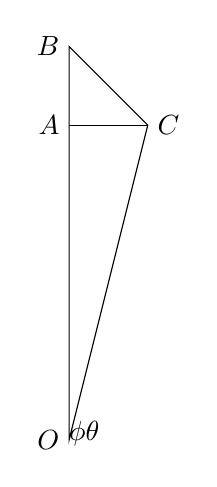
\begin{tikzpicture}
\coordinate [label=left:{$O$}] (O) at (0, 0);
\coordinate [label=left:{$A$}] (A) at (0, 4);
\coordinate [label=left:{$B$}] (B) at (0, 5);
\coordinate [label=right:{$C$}] (C) at (1, 4);

\draw (O)--(B)--(C)--cycle;
\draw (A)--(C);

\tkzLabelAngle(C,O,A){$\phi$};
\tkzLabelAngle[pos=0.4](A,B,C){$\theta$};
\end{tikzpicture}
\caption{Apparent speed of a moving object.}
\end{figure}

Let the body emit a signal at time $t_1$ when it is at $B$ and another one at
time $t_2$ when it is at $C$. Let the observer receive these signals at times
$t_1^\op$ and $t_2^\op$ respectively. If the signal travels at the speed of
light,
\begin{eqnarray}
t_1^\op &=& t_1 + d(O, B)c \label{c1e105} \\
t_2^\op &=& t_1 + d(O, C)c. \label{c1e106}
\end{eqnarray}
If $\delta t = t_2 - t_1$ then the distance $d(B, C) = v\delta t$, where $v$
is the speed of the emitter. The observer sees the body move from point $A$
to point $C$, a distance of $v\delta t\sin\theta$ in a time $\delta t^\op =
t_2^\op - t_1^\op$. Let $d(O, A)=D$. Then $d(O, B) = D + v\cos\theta\delta t$.
If $\phi$ is very small then $d(O, A) \approx d(O, C)$. Equations \eqref{c1e105}
and \eqref{c1e106} become
\begin{eqnarray}
t_1^\op &=& t_1 + Dc + v\cos\theta\delta t/c \label{c1e107} \\
t_2^\op &=& t_2 + Dc \label{c1e108}
\end{eqnarray}
so that $\delta t^\op = \delta t(1  + vc\cos\theta)$. The speed apparent to
the observer is 
\begin{equation}\label{c1e109}
v_\mu = \frac{v\sin\theta}{1 + (v/c)\cos\theta}.
\end{equation}
$v_\mu$ will exceed $c$ if
\[
v\sin\theta > c + v\cos\theta \Rightarrow v(\sin\theta - \cos\theta) > c
\Rightarrow \sin\theta - \cos\theta > \frac{c}{v},
\]
which can happen if $\pi/2 < \theta < \pi$.
\end{enumerate}
